\documentclass[letterpaper,11pt]{article}
\oddsidemargin -1.0cm \textwidth 17.5cm

\usepackage[utf8]{inputenc}
\usepackage[activeacute,spanish, es-lcroman]{babel}
\decimalpoint
\usepackage{amsfonts,setspace}
\usepackage{amsmath}
\usepackage{amssymb, amsmath, amsthm}
\usepackage{comment}
\usepackage{float}
\usepackage{amssymb}
\usepackage{dsfont}
\usepackage{anysize}
\usepackage{multicol}
\usepackage{enumerate}
\usepackage{graphicx}
\usepackage[left=1.5cm,top=2cm,right=1.5cm, bottom=1.7cm]{geometry}
\setlength\headheight{1.5em} 
\usepackage{fancyhdr}
\usepackage{multicol}
\usepackage{hyperref}
\usepackage{wrapfig}
\usepackage{subcaption}
\usepackage{siunitx}
\usepackage{cancel}
\usepackage{mdwlist}
\usepackage{svg}
\pagestyle{fancy}
\fancyhf{}
\renewcommand{\labelenumi}{\normalsize\bfseries P\arabic{enumi}.}
\renewcommand{\labelenumii}{\normalsize\bfseries (\alph{enumii})}
\renewcommand{\labelenumiii}{\normalsize\bfseries \roman{enumiii})}


\begin{document}

\fancyhead[L]{\itshape{Facultad de Ciencias F\'isicas y Matem\'aticas}}
\fancyhead[R]{\itshape{Universidad de Chile}}

\begin{minipage}{11.5cm}
    \begin{flushleft}
        \hspace*{-0.6cm}\textbf{FI1000-1 Introducción a la Física Clásica}\\
        \hspace*{-0.6cm}\textbf{Profesora:} Jocelyn Dunstan\\
        \hspace*{-0.6cm}\textbf{Auxiliar:} Alejandro Silva\\
        \hspace*{-0.6cm}\textbf{Ayudantes:} Macarena Muñoz \& Catalina Vargas\\
    \end{flushleft}
\end{minipage}

\begin{picture}(2,3)
    \svgpath{../}  % descomentar si se agrega a carpeta "auxiliares"/"ejercicios"
    \put(366, 10){\includesvg[scale=0.31]{img/dfi.svg}}
\end{picture}

\begin{center}
	\LARGE\textbf{Ejercicio \#6}\\
	\Large{Trabajo y energía}
\end{center}

\vspace{-1cm}
\begin{enumerate}\setlength{\itemsep}{0.4cm}

\rfoot[]{pág. \thepage}

\item[]

\item Una masa $M$ está atada al extremo de un resorte de constante $k$, adosado a una pared. La masa desliza sobre un plano horizontal cuyo coeficiente de roce cinético es $\mu$.

Inicialmente el resorte está comprimido a una distancia $\delta_0$ con respecto a su posición de equilibrio. En $t=0$ la masa se suelta, llegando a alcanzar una elongación máxima $\delta_1$, luego vuelve y alcanza una distancia máxima $\delta_2$ y así sucesivamente (ver Figura \ref{fig:ej6}).

Encuentre una relación entre $\delta_i$ y $\delta_{i+1}$.

\begin{figure}[H]
    \centering
    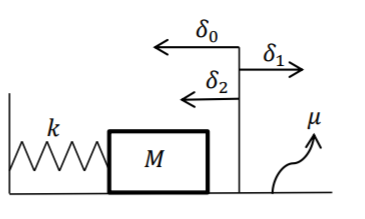
\includegraphics[width=10cm]{2021-2/img/ejercicios/imagen_ej6.png}
    \caption{Semana 9, vamos que se puede}
    \label{fig:ej6}
\end{figure}

Formulario:

\begin{equation}
    E_{final}-E_{inicial}=W_{roce}
\end{equation}

\begin{equation}
    E_{resorte}=\frac{1}{2}k(\Delta x)^2
\end{equation}

\begin{equation}
    W_{roce}=F_{roce} \cdot \Delta x
\end{equation}

\begin{equation}
    F_{roce}=\mu N
\end{equation}


% Para imágenes vectoriales -> el texto tiene que estar en LaTeX
% \begin{figure}[htbp]
%   \centering
%   \svgpath{../Imagenes/ejercicios}  -> .. irse pa'trás 
%   \includesvg{ej5.svg}
% \end{figure}

\end{enumerate}
\end{document}